\documentclass{article}
\usepackage{neb-macros}
\usepackage{tikz}
  \usetikzlibrary{patterns}

\begin{document}

\CheapTitle{Subrings}

\begin{center}
\framebox{Where can we find rings?}
\end{center}

Of course the difficult part of building a ring is coming up with the arithmetic -- the plus and times -- so that the ring axioms are satisfied. Well, suppose we already have a ring $R$ lying around. Perhaps we can use the fact that $R$ already has a nice plus and times to build new rings.

\begin{center}
\framebox{Given a ring $R$, how can we construct new rings out of the ``parts'' of $R$?}
\end{center}

The simplest way to do this is by taking a subset of $R$, and restricting the arithmetic on $R$ to that subset.

There is a potential obstacle to making this work, though; given a subset $S \subseteq R$ and two elements $x,y \in S$, \emph{a priori} we expect their sum $x+y$ to be in $R$, not necessarily in $S$. This is a problem! To avoid this, we single out the subsets of $R$ for which precisely this does not happen. That is, the subsets which are closed under the arithmetic on $R$.

\begin{center}
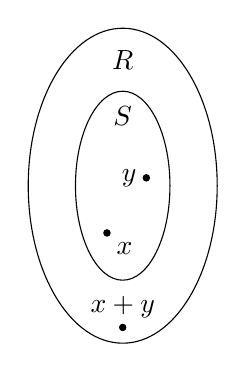
\begin{tikzpicture}[scale=0.4]
  \draw (0,0) ellipse (3 and 5);
  \node at (0,4) {$R$};
  \draw (0,0) ellipse (1.5 and 3);
  \draw [fill] (-0.5,-1.5) circle (0.1) node [below right] {$x$};
  \draw [fill] (0.75,0.25) circle (0.1) node [left] {$y$};
  \draw [fill] (0,-4.5) circle (0.1) node [above] {$x+y$};
  \node at (0,2.2) {$S$};
\end{tikzpicture}
\end{center}

\begin{dfn}[Subring]
Let $R$ be a ring and $S \subseteq R$ a subset. We say that $S$ is a \emph{subring} of $R$ if $S$ is closed under the operations in $R$. Specifically,
\begin{enumerate}
\item $0_R \in S$,
\item If $x,y \in S$ then $x+y \in S$,
\item If $x \in S$ then $-x \in S$, and
\item If $x,y \in S$ then $xy \in S$.
\end{enumerate}
If $R$ is unital, we say that a subring $S$ is \emph{unital} if in addition $1_R \in S$. 
\end{dfn}

\begin{prop}
If $R$ is a ring and $S \subseteq R$ a subring, then $S$ is itself a ring under the restricted operations on $R$.
\end{prop}

\begin{prop}[Subring Criterion]
Let $S \subseteq R$ be a subset. Then $S$ is a subring of $R$ if and only if $S$ is not empty and is closed under subtraction and multiplication. That is, $S$ is a subring of $R$ iff the following hold.
\begin{itemize}
\item $S \neq \varnothing$.
\item If $x,y \in S$ then $x-y \in S$.
\item If $x,y \in S$ then $xy \in S$.
\end{itemize}
\end{prop}

We have a slightly easier way to characterize \emph{unital} subrings.

\begin{prop}[Unital Subring Criterion]
Let $R$ be a unital ring. Then $A \subseteq R$ is a unital subring if and only if $1_R \in A$ and for all $x,y,z \in A$, $x-yz \in A$.
\end{prop}

\subsection*{Examples}

\begin{enumerate}
\item[$0$] Let $R$ be any ring. The subset $0 = \{0_R\} \subseteq R$ is a subring. (Show it!)

\item[$k\ZZ$] Let $k$ be a positive integer, and define $k\ZZ = \{ kt \mid t \in \ZZ \}.$ Then $k\ZZ \subseteq \ZZ$ is a subring, but is \emph{not} a unital subring.

\item[$aR$] More generally, let $R$ be any ring and $a \in R$. Then $aR = \{ ar \mid r \in R \}$ is a subring of $R$; similarly, $Ra = \{ ra \mid r \in R \}$ is a subring of $R$.

\item[$Z(R)$] Let $R$ be a ring. We define a subset of $R$ called the \emph{center} as follows. \[ Z(R) = \{ a \in R \mid ax = xa\ \mathrm{for\ all}\ x \in R \} \] That is, the center is the set of all ring elements which commute with every other element of $R$. For example, $0_R \in Z(R)$, since if $x \in R$ we have $0 \cdot x = 0 = x \cdot 0$. Then $Z(R)$ is a subring of $R$. If $R$ is unital, then $Z(R)$ is a unital subring.

\item[$S_1 \cap S_2$] Suppose $S_1, S_2 \subseteq R$ are (unital) subrings of $R$. Then $S_1 \cap S_2 \subseteq R$ is also a (unital) subring of $R$.
\end{enumerate}



\subsection*{Exercises}

\begin{enumerate}
\item Let $R = \ZZ$ and $S \subseteq R$ the set of all prime integers. Show that $S$ is \emph{not} a subring of $R$.

\item Let $R$ be a ring, and let $e \in R$ be idempotent. Show that \[ eRe = \{ ere \mid r \in R \} \] is a subring of $R$. Show that as a ring, $eRe$ is unital with $1 = e$. In particular, if $R$ is a unital ring and $e \neq 1_R$, then $S$ is not a \emph{unital subring}, even though it is a \emph{subring which is unital}, since in a unital subring $S$ we have $1_S = 1_R$.
\end{enumerate}

\end{document}
